\documentclass[12pt]{article}

\usepackage{lastpage} % Required to determine the last page for the footer
\usepackage{extramarks} % Required for headers and footers
\usepackage{graphicx} % Required to insert images
\usepackage{listings} % Required for insertion of code
\usepackage{courier} % Required for the courier font
\usepackage{color}

% Margins
\topmargin=-0.45in
\evensidemargin=0in
\oddsidemargin=0in
\textwidth=6.5in
\textheight=9.0in
\headsep=0.25in

\linespread{1.1} % Line spacing

\vspace{4em}

\newcommand{\Title}{Software Architecture Specification Document} % Assignment title
\begin{document}

	\begin{center}%
		\LARGE \bf \Title \\[2em]
		\Large {Project:}\\
		Financial markets simulation with multiple competing algorithmic trading entities.\\[0.7em]
		\Large {Client:}
		Cortical Systems\\[2em]
		\LARGE {\bf Group:}\\
			\begin{figure}[ht!]
				\centering
				
\includegraphics[scale=0.4]{Logo8.png}
			\end{figure}
			
		\Large {\bf Members:}\\[0.3em]
		\large
		Daniel Makgonta 12147100\\
		Moeletji Semenya 12349136\\
		Madimetja Shika 12127877\\[3em]
	
	\small Publication Date: 21 May 2014\\[0.5em]
	\small Version: 0.3		    
	\end{center}%
	
	\newpage		
	\large 
 	{\bf Change Log}\\[1em]
	\begin{tabular}{llll}
		Date & Name & Reason & Version \\
		13/05/2014 & Moeletji & Creation & 0.0 \\
		16/05/2014 & Moeletji & Adding functional requirements & 0.0 \\
		19/05/2014 & Daniel & Added Architectural Requirements & 0.0 \\
		21/05/2014 & Madimetja & Editing & 0.0 \\
		12/07/2014 & Daniel & Edited Architecure requirements & 0.1 \\
		15/07/2014 & Moeletji & Added to functional requirements & 0.1 \\
		22/07/2014 & Madimetja & Edited the document & 0.1 \\
		23/07/2014 & Daniel & Updated Architecure requirements & 0.1\\
		23/07/2014 & Moeletji & Updated functional requirements & 0.1\\
		27/07/2014 & Daniel & Revised architectural requiremets & 0.1\\
		28/07/2014 & Moeletji & Added function requirements & 0.1\\
		29/07/2014 & Madimetja & Edited and Reviewd document & 0.1\\
		31/07/2014 & Madimetja & Added vision and scope sections & 0.1\\
		01/08/2014 & Moeletji & Added final images and compiled document & 0.2\\
		21/08/2014 & Madimetja &  Updated Class Diagram document & 0.2\\
                20/08/2014 & Daniel & Added section for GUI and pictures & 0.3\\
                22/08/2014 & Daniel & Edited Architectural Constraints & 0.3\\
	\end{tabular}
	
	\newpage
	\tableofcontents
				  
		\newpage
			\section{Vision and Scope}
				\subsection{Vision}
				The vision is to create a system that simulates the activities of a real-world financial market and the entities involved, while allowing interaction from both real-word and virtual entities.
				
				\subsection{Scope}
				The proposed system is a financial markets simulator system which will allow trading entities to:
				\begin{itemize}
				\item trade instruments through the system as they would in a real-world financial market while adhering to free market principles,
				\item observe and follow trends in the market through the system by means of observing technical analysis patterns and indicators. This would furthermore provide entities with information on when best to enter or exit the market,
				\item compete with each other by assessing the profit and loss thy make.
				\end{itemize}
				
				In particular, apart from allowing the participants to compete with each other in terms of the profits or loss they make, the system will allow the following specific activities for participants:
				
				\begin{itemize}
				\item Sellers (Offerors)
					\begin{itemize}
					\item make offers to sell shares.
					\item sell shares to buyers.
					\end{itemize}
				\item Buyers (Bidders)
					\begin{itemize}
					\item propose bids to buy shares.
					\item search for shares on sale.
					\item buy shares on sale.
					\end{itemize}
				\item Companies
					\begin{itemize}
					\item Enter the market (system) and list stocks on the market (system).
					\end{itemize}
				
				\end{itemize}
				\subsection{Limitations/Exclusions}
				The project scope explicitly excludes and/or is limited in the following manner:
				\begin{itemize}
				\item Stock-brokers will not be explicitly active in the system as individual separate independent entities. The responsibilities of the stock-broker will be handled and performed by the matching engine and relevant market managers.
				\end{itemize}
					  
				  
		\newpage
		This part of document discusses the requirements around the software infrastructure within which the application functionality is to be developed. 
		\section{Access channel requirements}
		The system will be accessible by human users through the following front-end channels:
		\begin{itemize}
		\item From a stand-alone Java application interface. The system will be accessible from any desktop or laptop once the appication is installed on the device.
		\end{itemize}
		
		\section{Quality Requirements}
			\subsection{Usability}
			\begin{itemize}
			\item The system should be usable in that the architecture should provide the neccessary components to view and interact with the system.
			\end{itemize}
			\subsection{Scalability}
			\begin{itemize}
			\item If need be, the system should allow for independent entities operating from independent machines to participate in the market. i.e. The system should allow for at least two (2) participants to partiipate in the market from separate machines.
			\item The system should allow for concurrent trading between at least two (2) separate machines.
			\end{itemize}
			\subsection{Performance}
			\begin{itemize}
			\item In the case that multiple physical machines are used, the architecture should allow offers and trades to be communicated to and from the matching engine via the network in under 50 milliseconds (1/20 of a second). 
			\end{itemize}
		\section{Integration Requirements}
		The system is self-contained and there is no need for integration with other external systems or components.
		\section{Architectural Constraints}
		\begin{itemize}
		\item In order to minimize cost and complexity, the system can be developed to run and operate on a single physical machine. 
		\end{itemize}
	
        \newpage
                \section{Architectural requirements}	    
			    \subsection{Architectural scope}	

                                \begin{itemize}
                                     \item Concurrent threading execution of Market Participants for a realistic simulation.
                                     \item A relational database will be the persistent infrastructure used to record data.
                                     \item Full API of the system will be available.
                                 \end{itemize}

			    \subsection{Quality requirements}	
			    	\subsubsection{Security}
			    	\begin{itemize}
			    		\item Only system administrators may tweak trading algorithms or matching engine to follow current trends within the stock market.
                                        \item The system allows anonymity in terms of no buyer or seller can view what another buyer or seller�s activities.
                                        \item Matching engine is only allowed to be accessed directly by system administrators. 
                                        \item The matching engine is abstracted to the buyers and sellers of the system. 
                                        \item System administrators are not allowed to participate in the trading simulation.
			    	\end{itemize}	
			    		
			    	\subsubsection{Auditability}
			    	\begin{itemize}
				    	\items One can query any Market Data generated within the system, this includes the user who made the change, the data that was changed, the new and old values of the data, as well as when the data was changed
			    	\end{itemize}
			    	
			    	\subsubsection{Testability}
			    	\begin{itemize}
			    		\item All services provided by the system are testable with unit tests, that the service is provided if all pre-conditions are met (i.e. that no exception is raised except if one of the pre-conditions for the service is not met), and that all post-conditions hold true once the service has been provided.
			    	\end{itemize}
			    
			    	\subsubsection{Usability}
			    	\begin{itemize}
			    		\item System will support up to 40 Market Participants and 3 Stock Markets.
                                        \item The system will be presented in the English language, and with further development will cater for other popular languages.
                                        \item The Graphical User Interface will use design principals and usability goals from interaction design theoretical frameworks to increase the ease of using the system for the first time.
                                        \item All calculations will be abstracted for the users and the Graphical User Interface will only show averages and final results to the user.
                                \end{itemize}
			    
			    	\subsubsection{Scalability}
			    	\begin{itemize}
			    		\item The system will be able to use 10 trading algorithms and allow more algorithms to be plugged in at a later stage.
                                        \item The system will be able to concurrently trade with 20-40 Market Participants trading 1-3 different Market Entities effectively and accurately according to the business rules of the system.
                                        \item The system will have an API that can be used with different interfaces. 
                                \end{itemize}
			    	
			    	\subsubsection{Performance}
			    	\begin{itemize}
			    		\item The matching engine will return matches in less than 0.5 seconds
                                        \item Reporting of the market will be displayed in less than 5 seconds
                                        \item The buyers and sellers will be able the concurrently interact with the market simulation and this would take less than 0.5 second
                                \end{itemize} 
			    	    		
                            \subsection{Access Channel Requirements}
                                 The system is a stand-alone system and does not integrate with any other systems.
                                 The system will be accessible by human users through the following channel:
                                         \begin{itemize}
                                             \item From any system that contains a JVM (Java Virtual Machine).
                                         \end{itemize}
			   			
                            \subsection{Architectural Constraints}	
                                    \begin{itemize}
                                            \item System runs on a JVM
                                            \item System uses MySQL as its database
                                            \item Operating systems: Windows, Linux, Mac OS X
                                    \end{itemize}						    	    
		\subsection{Architectural patterns/styles}
                                \begin{itemize}
                                    \item \textbf{Interface Segregation:} system has an API that can be used by other interfaces other than its native interface.
                                    \item \textbf{Singleton:} the system only allows an instance of one Stock Exchange to prevent overwhelming the system�s resources. With improved system the system may be adapted to work with more than one stock exchange
                                    \item \textbf{Polymorphism:} All strategies inherit from a base strategy, but all sub-types have different strategies.
                                    \item \textbf{Encapsulation:} All Stocks are encapsulated by their managers to allow for further extensibility of the functionality.
                                    \item \textbf{Observer:} Market Participants will be notified of changes in Matching Engine. 
                                    \item \textbf{Message Queue:} Market Participants will send Messages in the form of a Message Queue to the Matching Engine to ensure fairness.
                                \end{itemize}
                \subsection{Architectural Tactics and Strategies} 
                    \begin{itemize}
                        \item Full separate functional API allows for pluggable application interfaces.
                        \item Multi-Threading Market Participants allow for real-time simulation.
                    \end{itemize}

                \subsection{Technologies}
                    \begin{itemize}
                        \item \textbf{Built Environment:} Maven
                        \item \textbf{Software:} Java
                        \item \textbf{IDE:} Netbeans
                        \item \textbf{Database:} MySql
                        \item \textbf{Programming Languages:} Java
                        \item \textbf{Business logic:} Java
                        \item \textbf{Interface:} Java
                    \end{itemize}

		\section{Architectural Constraints}
		\begin{itemize}
		\item In order to minimize cost and complexity, the system can be developed to run and operate on a single physical machine. 
		\end{itemize}

        \newpage
	\section{User Interface}
            A user will create stocks and market participants with relevant data and 
            will the simulator by selecting which market participants trades in which stocks.

            \begin{figure}[th]
                            \centering
                            
\includegraphics[scale=0.6]{./menu}
                            \caption{Menu of Interface}
                            \label{Menu}
            \end{figure}
            \\
            \begin{figure}[th]
                            \centering
                            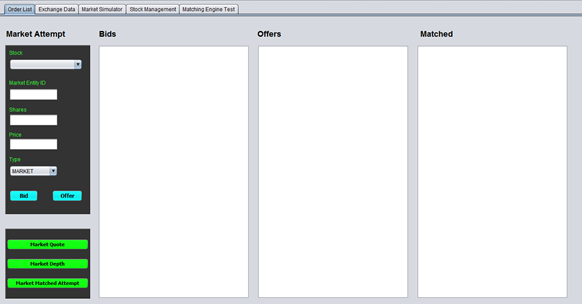
\includegraphics[scale=0.6]{./matchingengine}
                            \caption{Matching Engine of Interface}
                            \label{Matching Engine}
            \end{figure}
            \\
            \begin{figure}[th]
                            \centering
                            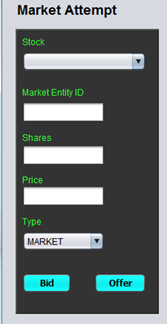
\includegraphics[scale=0.6]{./marketentryattempt}
                            \caption{Create Market Entry Attempt}
                            \label{Market Entry Attempt}
            \end{figure}
            \\
            \begin{figure}[th]
                            \centering
                            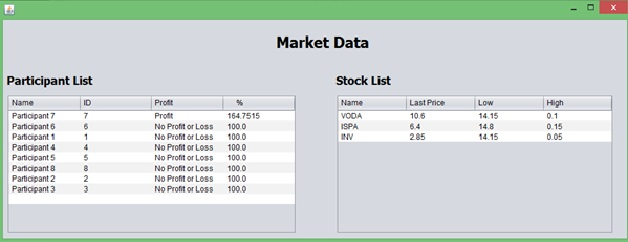
\includegraphics[scale=0.6]{./marketdata}
                            \caption{View Market Data}
                            \label{Market Data}
            \end{figure}
            \\
            \begin{figure}[th]
                            \centering
                            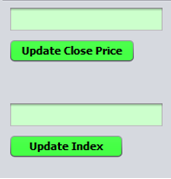
\includegraphics[scale=0.6]{./priceupdates}
                            \caption{Set Price Updates}
                            \label{Price Updates}
            \end{figure}
            \\
            \begin{figure}[th]
                            \centering
                            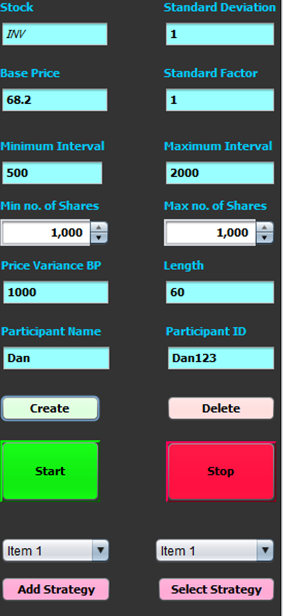
\includegraphics[scale=0.6]{./marketparticipant}
                            \caption{Create and Manage Market Participants}
                            \label{Market Participants}
            \end{figure}
            \\
            \begin{figure}[th]
                            \centering
                            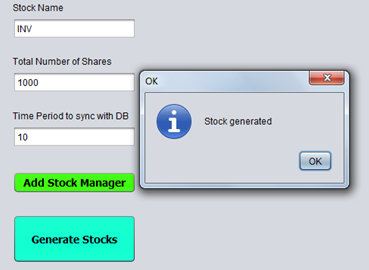
\includegraphics[scale=0.6]{./createstocks}
                            \caption{Create or Generate Stocks}
                            \label{Stocks}
            \end{figure}
            \\
            \begin{figure}[th]
                            \centering
                            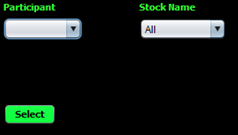
\includegraphics[scale=0.6]{./marketparticipantdata}
                            \caption{View Market Participant Data}
                            \label{Market Participants}
            \end{figure}
            \\
            \begin{figure}[th]
                            \centering
                            \includegraphics[scale=0.6]{./tradingmarketparticipants}
                            \caption{View Trading Market Participants
                            \label{Market Participants}
            \end{figure}
            \\

	\newpage		    		    		    			    	
	\section{Functional requirements and application design}
		\subsection{Introduction}	
		This part of the document outlines the functional requirements of the \textit{Financial market simulation} at the different levels of granularity. In the deisgn of the system we followed the SOLID design principles.
		
			\begin{figure}[th]
			\centering
			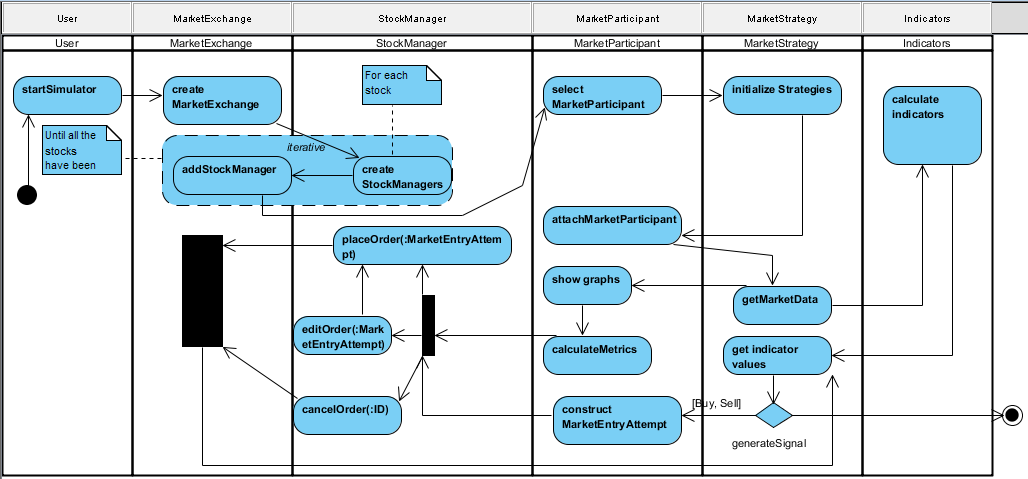
\includegraphics[scale=0.6]{./activity}
			\caption{A high level activity diagram of the Financial Market Simulator}
			\label{domain objects}
			\end{figure}
		\pagebreak			    
		\subsection{Required functionality}	
				\subsubsection{Matching Engine}
				\begin{itemize}
					\item Requirement Prioritization: Critical
					\item Requirement Source: Client 	
					\item Requirement Level: High
				\end{itemize}
			 	
				\textbf{Pre-condition} :If no MarketEntryAttempts(bids and offers) are entered.\\
			 	\textbf{Post-conditions} : A MatchedMarketEntryAttempt of a trade.\\ 
			 	\textbf{Request Data Structure} : MarketEntryAttempt object.\\
			 	\textbf{Result Data Structure} : MatchedMarketEntryAttempt object.\\
			 	
				This is the core of the whole system. The following functionality should be provided:
					\begin{itemize}
						\item Provide a mechanism for accepting and maintaining market depth of bids and offers.
						\item Match the different types of market orders(e.g. primarily bids and offers).
						\item Notifying the relevant market participants of the matches involved in(if any).
						\item Report market data back to market participants.
					\end{itemize}
				So all bids and offers will be dealt with by the matching engine.	
				
						\begin{figure}[th]
						\centering
						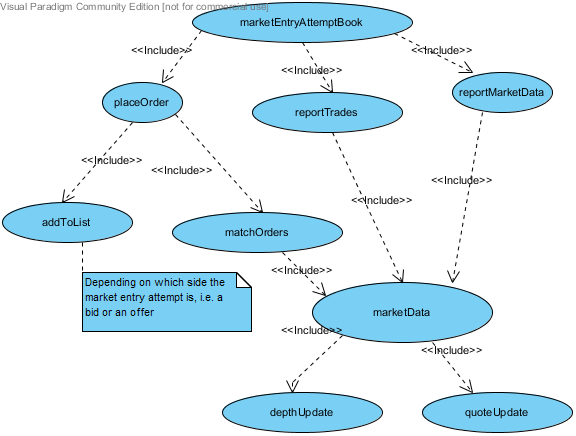
\includegraphics[scale=0.8]{./matching_engine_use_case}
						\caption{Use case for the matching engine}
						\label{matching engine use case}
						\end{figure}
				\pagebreak
				
				\subsubsection{Keep track of the bids and offers}
						\begin{itemize}
							\item Requirement Prioritization: Critical
							\item Requirement Source: Client 
							\item Requirement Level: High	
						\end{itemize}
						
						\textbf{Pre-condition} :If no MarketEntryAttempts(bids and offers) are entered.
						If the price or quantity of shares is zero.\\ 
						\textbf{Post-conditions} : An ordered bids and offers stacks.\\ 
						\textbf{Request Data Structure} : MarketEntryAttempt object.\\
						
						The bids and offers should be stored in different stacks in the appropriate order. The offers will be stored in ascending order and the  bids will be stored in descending order in terms of the price per share value. The market entry attempt will be stored if and only if their is no matching order(in terms of price) on the opposite stack.\\
						
						This is an important part of the system as the correct order of the bids and offers must be stored because the order of the MarketEntryAttempts(bids and offers) is crucial to the functioning of the system.
						
						\begin{figure}[th]
									\centering
									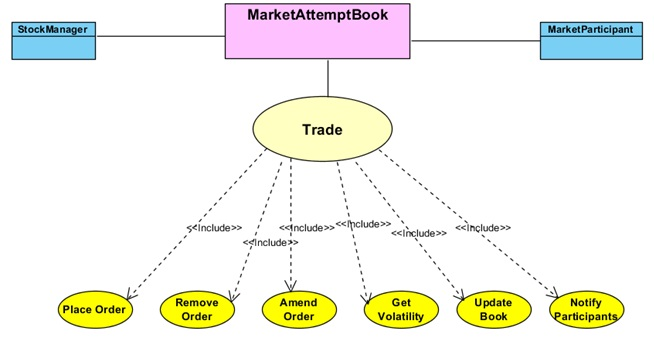
\includegraphics[scale=0.6]{./USE_CASE_Market_Attempt_Book_Financial_Market_Simulator}
									\caption{The class with the market depth}
									\label{domain objects}
						\end{figure}
												
				\subsubsection{Provide persistent storage for the market data generated by the system}
								\begin{itemize}
									\item Requirement Prioritization: Critical
									\item Requirement Source: Client 
									\item Requirement Level: High	
								\end{itemize}
								
								\textbf{Pre-condition} :If no trades occur.\\
								\textbf{Post-conditions} :Records of the trades that occured stored in the database.\\ 
							 	\textbf{Request Data Structure} : MatchedMarketEntryAttempt object.\\
							 	
								The financial market simulator is going to generate its own historical data so a mechanism needs to be put in place to store the market data of trades and other information used in generating trading events. These trading events will be using technical indicators and chart patterns.\\
								
								A relational database will be used for the persistent storage of market data using the MySql server and a MySql connector to connect to the system. With this in place all the market data can be gathered in order to be analysed later to see how the financial market is behaving in certain circumstances.
								
				\subsubsection{User Interfaces for the market participants and the whole financial market}
								\begin{itemize}
									\item Requirement Prioritization: Critical
									\item Requirement Source: Client 
									\item Requirement Level: High	
								\end{itemize}
								
								\textbf{Pre-condition} :If no trades occur.\\
								\textbf{Post-conditions} :Records of the trades that occured stored in the database.\\ 
								\textbf{Request Data Structure} : MatchedMarketEntryAttempt object.\\
									
								This requirement should provide the following user interfaces:
									\begin{itemize}
										\item  For displaying the various metrics of the performance of any selected market participant for comparing the different algorithms' performance.
										\item For showing the full market depth and matching orders by the matching engine.
									\end{itemize}
									
									For any participant, their interface should display all the participant's market data and whether the participant is making a profit or a loss. 
									The other part of the user interface will display all the activity going on in the market to see how the market it performing at that point in time.								
					
				\subsubsection{Calculating technical indicators for trading strategies}
						\begin{itemize}
							\item Requirement Prioritization: Critical
							\item Requirement Source: Client
							\item Requirement Level: High 	
						\end{itemize}
						
				\textbf{Pre-condition} :If there is no data available(as in trades) .\\
				\textbf{Post-conditions} : A value(s) calculated by the technical indicator.\\ 
						
				Technical indicators are used for analysing and interpreting market behaviour. This ranges from analysing the price of a stock or the number of shares traded or the trend of a certain share. The indicators generate value(s) and are interpreted so that they can be used by the strategies which will decide whether to enter(bid) or exit(offer) the market.\\
				Some of the indicators use each other to compute more complex technical indicators. So far 13 technical indicators have been implemented(*A library will be used if/when a suitable one is found).\\
				They are:
				\begin{itemize}
					\item Simple Moving Average(SMA)
					\item Exponential Moving Average(EMA)
					\item Negative Directional Index(NDI) 
					\item Positive Directional Index(PDI)
					\item Negative Directional Movement(NDM)
					\item Positive Directional Movement(PDM)
					\item Relative Strength Index(RSI)
					\item Moving Average Convergence Divergence(MACD)
					\item Average Directional Index(ADX)
					\item Average True Range(ATR)
					\item Volatility(Standard deviation)
					\item Bollinger Bands
					\item Stochastic Oscillator(SO)	
				\end{itemize} 								
				
				\subsubsection{Allow for at least 20 market participants}
				\begin{itemize}
					\item Requirement Prioritization: Critical
					\item Requirement Source: Client
					\item Requirement Level: High 	
				\end{itemize}
				Enable multiple market participants to be active in the market and allow for concurrent bids and offers to be placed. With this functionality, we can see how the market performs under certain(e.g. conditions when a stock is trending or when the market is liquid). \\
				
				Participants will use the trading strategies implemented in order to compete with each other in the financial market to see which ones perform better or not in terms of profit and loss. 
				
				\begin{figure}[th]
								\centering
								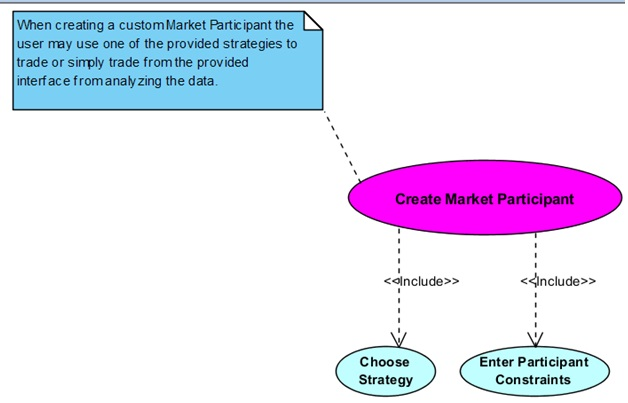
\includegraphics[scale=0.6]{./USE_CASE_Create_Market_Participant_Financial_Market_Simulator}
								\caption{A use case for creating a market participant.}
								\label{domain objects}
				\end{figure}
				
				\subsubsection{Algorithmic trading entities(strategies)}
				\begin{itemize}
					\item Requirement Prioritization: Critical
					\item Requirement Source: Client 	
					\item Requirement Level: High
				\end{itemize}
				Since there are multiple participants who will be competing in the market, we need to see how trading stategies perform in different market conditions. \\
				
				Each entity will need to do the following:
				\begin{itemize}
						\item Process market data and trading events from the matching engine
						\item Decide the entry or exit point into the market using data from the matching engine.
				\end{itemize}
					
				These are the different number of trading strategies that would be implemented by the developers. Different variations of trading strategies will be implemented(with the help of technical indicators). Each trading strategy will be able to process market data in order to use the information generated from the process and will generate a trading event(either a bid or offer). The trading algorithms will be able to remove bids and offers.\\
				
				So far 5 trading strategies have been implemented, namely: Crossover, Moving Average Crossover, Price EMA Crossover, Price SMA Crossover and the Moving Average Envelope. 
				\subsubsection{Generate trading events }
				\begin{itemize}
					\item Requirement Prioritization: Critical
					\item Requirement Source: Client 	
					\item Requirement Level: High
				\end{itemize}  
				
				The system should be able to generate bids and offers. The participant will have a mechanism(trading strategies) to decide how much to offer or bid and the quantity of shares. This requirement is strongly linked with previous requirement.	 
				
			\subsubsection{A mechanism for delivering messages about market events}
			\begin{itemize}
					\item Requirement Prioritization: Critical
					\item Requirement Source: Client 
					\item Requirement Level: High	
			\end{itemize}
			
			Messages about the last traded price need to be delivered to the other relevant market participants in order for them to have the latest information on whats happening in the market. The MarketEntryAttemptBook will deliver the messages to market participants and other components of the system that will need the latest data for computatoin purposes. All the market participants which are trading a particular instrument will be informed of what the other participants are doing.
			
			\subsubsection{Simulate the financial market}
			\begin{itemize}
				\item Requirement Prioritization: Critical
				\item Requirement Source: Client 
				\item Requirement Level: High	
			\end{itemize}
						
			The system needs to be able to simulate(without input from the user) in order to evaluate the trading algorithms(strategies) and market participants performances. The range for the prices and shares will be specified so that the financial market is controlled and trends can be spotted. 
			
			A user can manually envoke market events via the user interface into the financial market.
			
			\begin{figure}[th]
			\centering
			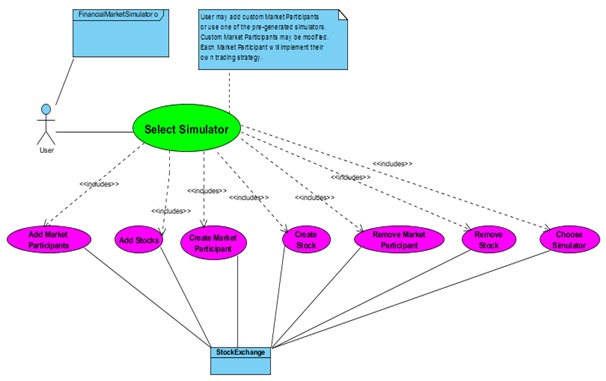
\includegraphics[scale=0.8]{./USE_CASE_Select_Simulator_Financial_Market_Simulator}
			\caption{A use case for showing how the simulator will be set up.}
			\label{domain objects}
			\end{figure}
				
			\begin{figure}[th!]
			\centering
			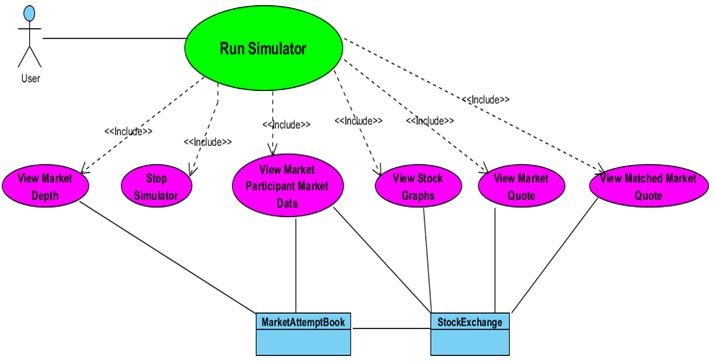
\includegraphics[scale=0.8]{./USE_CASE_Run_Simulator_Financial_Market_Simulator}
			\caption{A use case for showing what services will be available once the simulator is running.}
			\label{domain objects}
			\end{figure}
	
			\subsubsection{Provide a concurrent message queue between market participants and the matching engine}
			\begin{itemize}
				\item Requirement Prioritization: Important
				\item Requirement Source: Client 
				\item Requirement Level: Medium	
			\end{itemize}
			In order to have market participants decoupled from the matching engine,  the participants will communicate with the matching engine using a message queue interface. All the participants would do is place an order onto the message queue and the matching engine will be responsible for taking the message and process the request.
			
			\subsubsection{Allow the matching engine to broadcast market updates to all market participants using a message queue}
			\begin{itemize}
				\item Requirement Prioritization: Important
				\item Requirement Source: Client 
				\item Requirement Level: Medium	
			\end{itemize}
			The matching engine will be interacting with the message queue interface. After every state(a new order or a trade has occured or an order has been edited) change the matching engine will broadcast this change to all the market particpants by placing a message on the meassage queue.
			
			\subsubsection{Load market participants from persistent storage}
			\begin{itemize}
				\item Requirement Prioritization: Nice to have
				\item Requirement Source: Grape Team 
				\item Requirement Level: Medium	
			\end{itemize}
			Enable users to load market participants from persistent storage with their preferences as it can get tiring to enter a new market everytime one runs the system. 
			
			\subsubsection{Provide graphical representation of the data generated}
			\begin{itemize}
				\item Requirement Prioritization: Nice to have
				\item Requirement Source: Grape Team 
				\item Requirement Level: Medium	
			\end{itemize}
			Allow users who use the system to be able to see graphs(e.g. line graphs) of the calculated data(i.e technical iindicators) in order to see how the financial market and individual instruments are performing.
					  
		\subsection{Domain Objects}	
		See the last page.
								
			The strategy design pattern will be used for implementing the different trading algorithms to provide pluggability.
			And the observer design pattern will be used for the event handling of delivering messages about the activity in the financial market.
		\clearpage 
		\newpage	
			\begin{figure}[th]
			\centering
			\vbox{\vspace{-5em}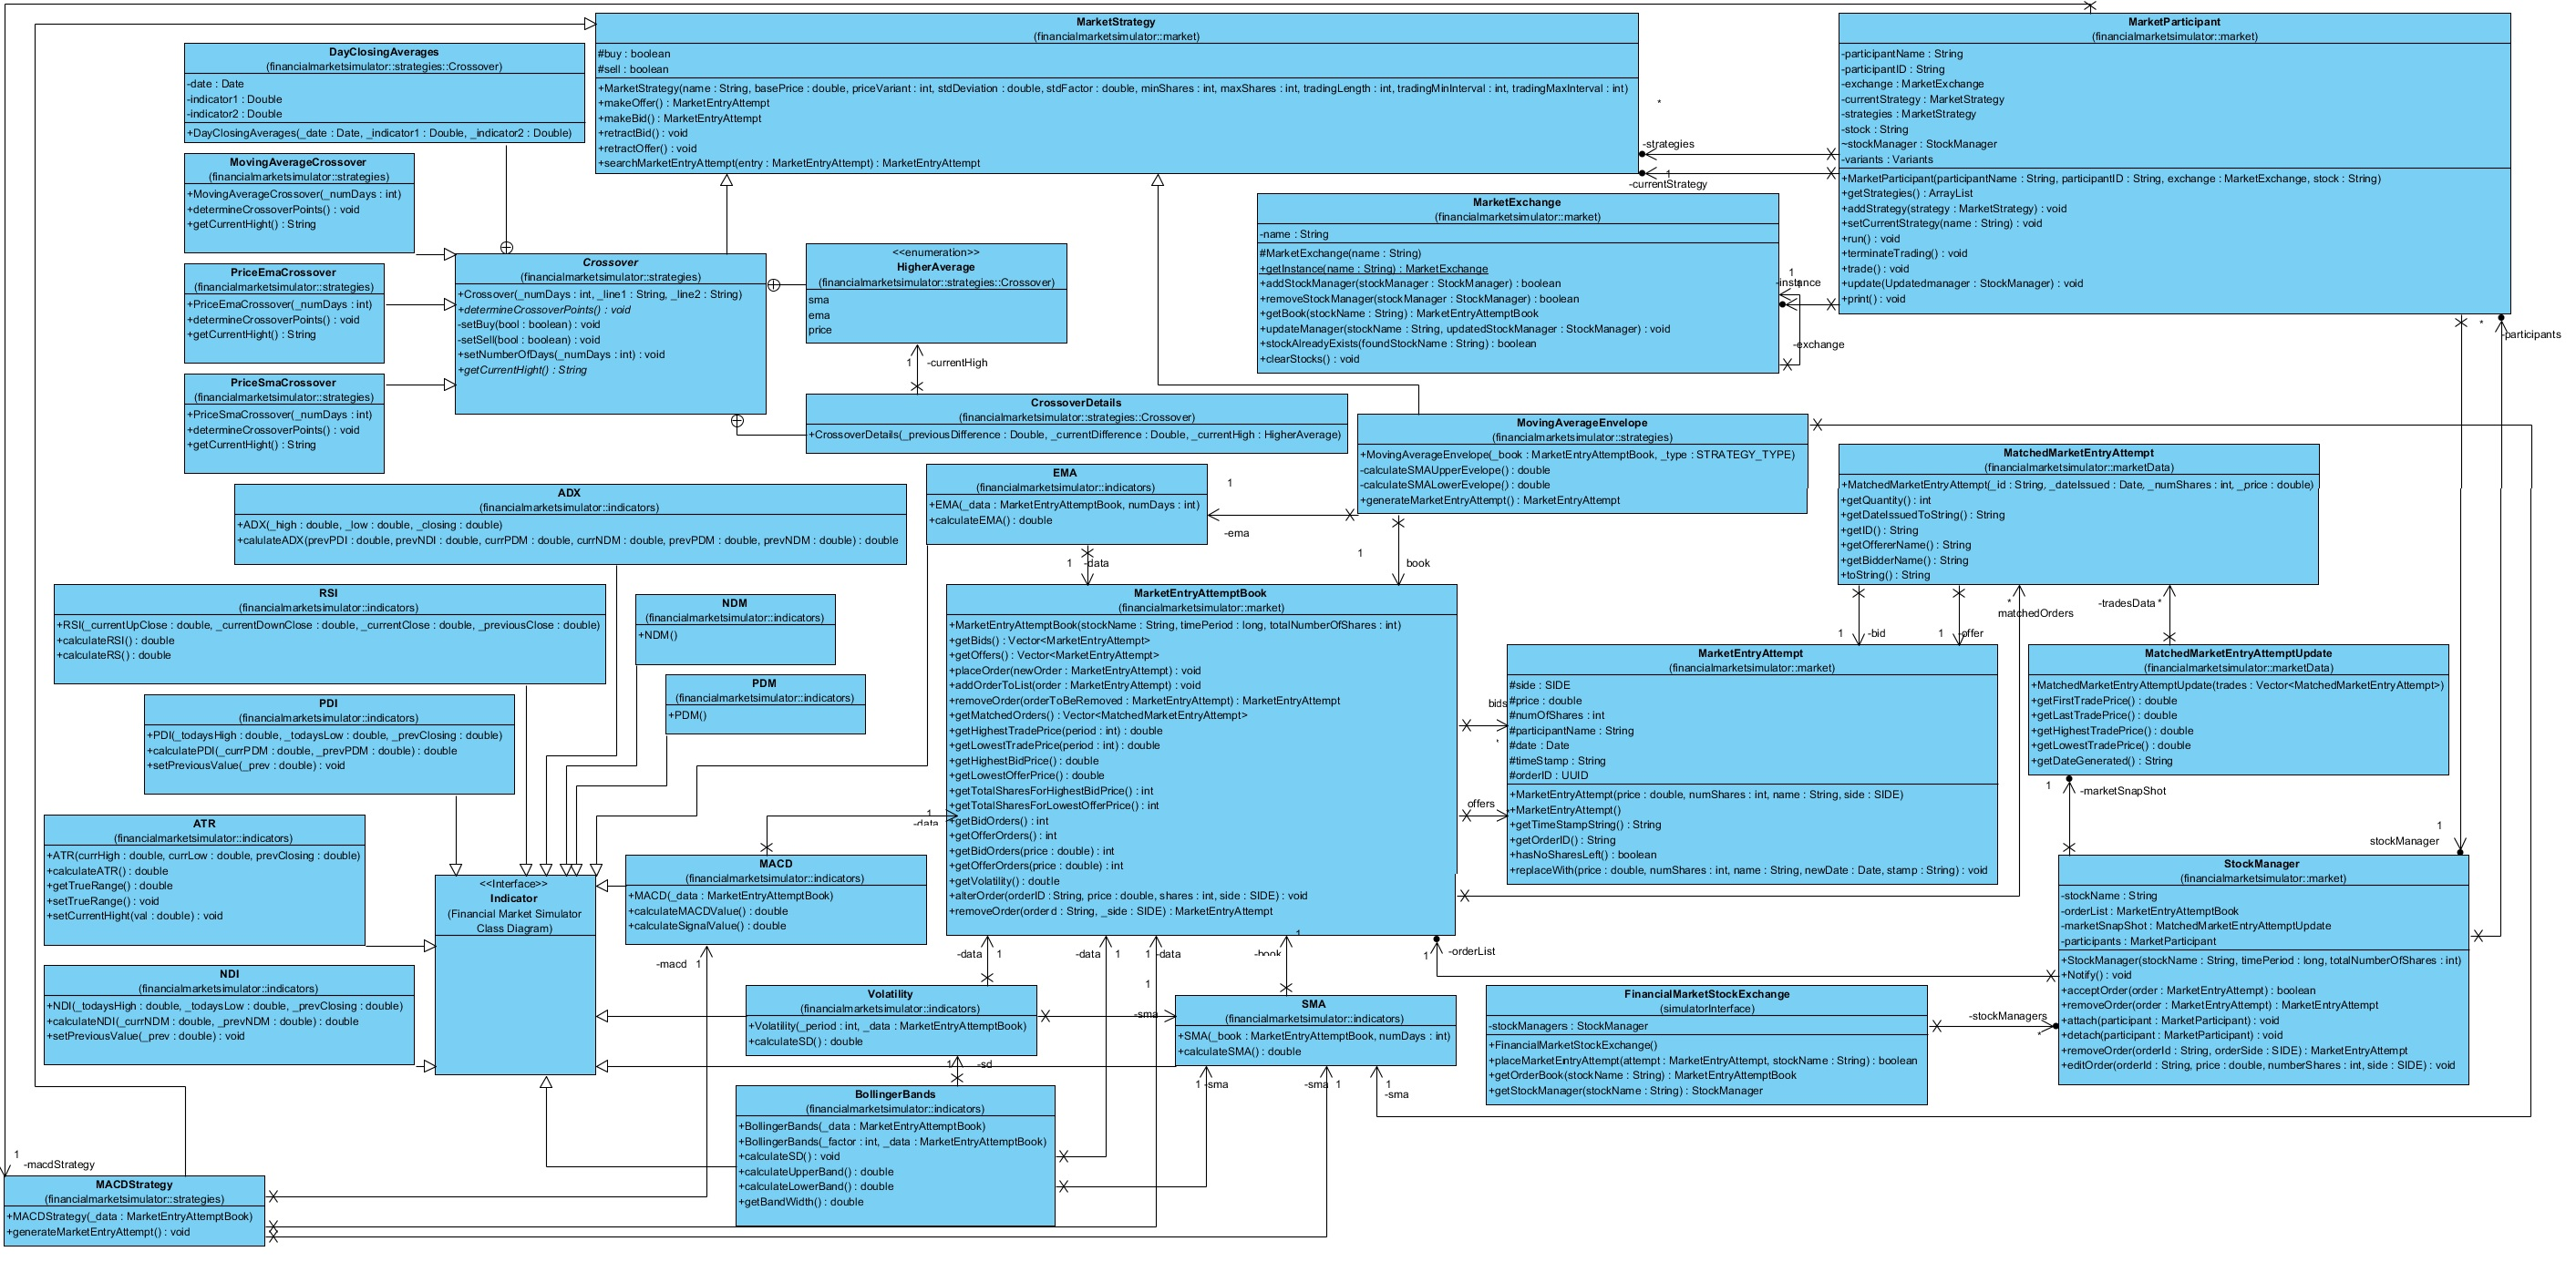
\includegraphics[scale=0.35, angle=90]{./ClassDiagram.jpg}}	
			\caption{Class diagram of the system so far}
			\label{domain objects}
			\end{figure}
		
	\clearpage	
	\newpage				
	\section{Glossary}	
		\begin{itemize}
			\item \textbf{Order}: An instruction from a participant to either put in an offer or a bid.
			\item \textbf{Market data}: Data reflecting current trading information to include pricing and volume and other additional information related to the trade.
			\item \textbf{Match}: When an offer and a bid have the same price.
			\item \textbf{Trading Event} Entering the market(placing an bid) or exiting the market(placing an offer). 
			\item \textbf{Volume}: A measure of activity i.e. the total number of shares one(a participant) has. 
		\end{itemize}				    			    			    		
\end{document}